\documentclass[11pt]{article}
\usepackage{preamble}
\titleformat*{\section}{\Large\bfseries}

\title{CISC 3220 Homework Assignment 2}
\author{Rachel Friedman}
\date{February 9, 2020}

\begin{document}
\maketitle

\section*{Question 1}\nointerlineskip
\noindent \rule{\linewidth}{0.01pt}\\
\noindent Use mathematical induction to establish that for every positive integer $n$:\\
\begin{equation*}
\sum_{i=1}^n  \frac{1}{(4i+1)(4i-3)} = \frac{n}{4n+1}
\end{equation*}

\noindent \textbf{Base case:} $n=1$
\begin{flalign*}
L(1)&=\sum_{i=1}^1  \frac{1}{(4(1)+1)(4(1)-3)} = \frac{1}{5}\\[3pt]
R(1)&=\frac{1}{4(1)+1}= \frac{1}{5}\\[6pt]
\text{Evidently, }L(1) &= R(1)\\
\end{flalign*}
\textbf{Inductive  Step:}  For every $k\in{N^+}$, if $L(k)=R(k)$, then $L(k+1)=R(k+1)$.\\

Let $k\in{N^+}$. Suppose $L(k)=R(k)$.\\
\begin{flalign*}
L(k+1)&=\sum_{i=1}^{k+1}  \frac{1}{(4(k+1)+1)(4(k+1)-3)} \\[6pt]
&=\sum_{i=1}^{k}  \frac{1}{(4k+1)(4k-3)} + \frac{1}{(4(k+1)+1)(4(k+1)-3)}\\[6pt]
&=\frac{k}{4k+1} + \frac{1}{(4k+5)(4k+1)}&&\textit{by Inductive Hypothesis}\\[6pt]
&=\frac{k(4k+5)}{(4k+5)(4k+1)} + \frac{1}{(4k+5)(4k+1)}\\[6pt]
&=\frac{4k^2+5k+1}{(4k+5)(4k+1)} = \frac{(4k+1)(k+1)}{(4k+5)(4k+1)} = \frac{k+1}{4k+5}\\[6pt]
&= \frac{k+1}{4(k+1)+1}\\[6pt]
&=R(k+1)
\end{flalign*}

\bigskip
\noindent This establishes that for every $k \in {N^+}$, if $L(k) = R(k)$, then $L(k + 1) = R(k+1)$.\\

\newpage
\section*{Question 2}\nointerlineskip
\noindent \rule{\linewidth}{0.01pt}
Use mathematical induction to establish $7^n - 2^n $ is divisible by 5 for every positive integer $n$.\\

\noindent \textbf{Base case:} $n=1$
\begin{flalign*}
7^1 - 2^1 = 5, \text{which is clearly divisible by 5}\\
\end{flalign*}
\textbf{Inductive  Step:} 
For every $k\in{N^+}$, if $p(k)$ is true, then $p(k+1)$ is true.\\

Let $k\in{N^+}$. Suppose proposition $p(k)$ is true. Verify that $p(k+1)$ is true:
\begin{flalign*}
 & 7^{k+1} - 2^{k+1}\\
&=(5+2)\cdot7^k - 2\cdot2^k\\[4pt]
&=5\cdot7^k +2(7^k -2^k)
\end{flalign*}
The first term ($5\cdot7^k$) is being multiplied by 5, and is therefore divisible by 5.\\
The second term ($2(7^k -2^k)$) is divisible by 5, according to the inductive hypothesis.\\
Hence, 7$^n - 2^n$ is divisible by 5 for every positive integer $n$.\\
\newpage
\section*{Question 3}\nointerlineskip
\noindent \rule{\linewidth}{0.01pt}
Consider the sequence (S$_n$)$_{n=0}^{\infty}$ for which $s_0 = s_1 = 1$ and for every integer $n\geq2$:
\[
s_n = s_{n-1} + 2s_{n-2}.
\]
a) Calculate the value of $s_6:$\\
\begin{flalign*}
&s(0) = 1\\
&s(1) = 1\\
&s(2) = s(1) + 2s(0) = 1 + 2(1) = 3\\
&s(3) = s(2) + 2s(1) = 3 + 2(1) = 5\\
&s(4) = s(3) + 2s(2) = 5 + 2(3) = 11\\
&s(5) = s(4) + 2s(3) = 11 + 2(5) = 21\\
&s(6) = s(5) + 2s(4) = 21 + 2(11) = 43\\
\end{flalign*}
%\indent $s_6 = 43$. \\
%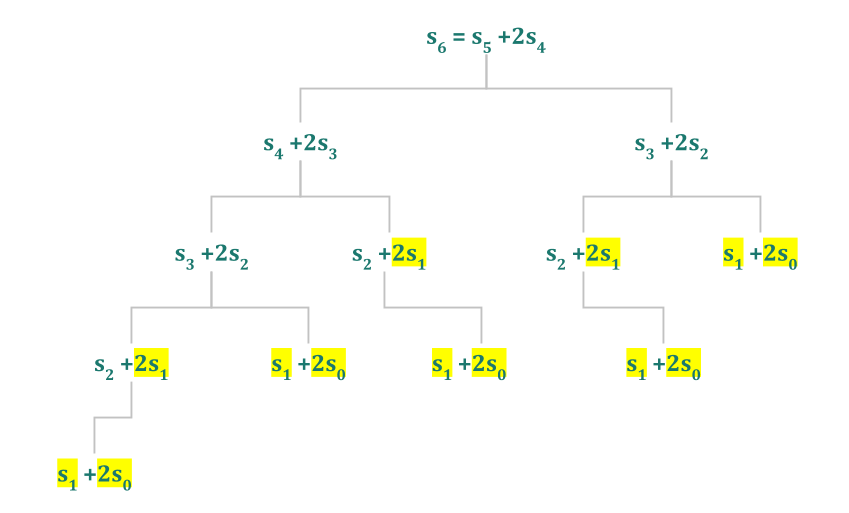
\includegraphics[scale=.4]{asst2_ques3}\\
\begin{comment}
\Tree[.t6 [.t5  [.t4 [.t3x ]
                      .t2]  
                [.t3 [.t2 [.N  ]]]]]
          [.t4r [.t3g ]
                [.t2g [.t1 [.t0 ]
                           [.t6 [.Deg \textit{really} ]
                                [.A\1 [.A \textit{simple} ]
                                      \qroof{x}.CP ]]]]]]
\end{comment}

\noindent b) Prove that all terms of the sequence (S$_n$)$_{n=0}^{\infty}$ are odd.\\

\noindent \textbf{Base cases}:  $S(0) = 1$, which is odd.\\ 
\indent \indent \indent \indent$S(1) = 1$, which is odd.\\

\noindent \textbf{Inductive Hypothesis}: $S(i)$ is odd for $ 0\leq i \leq k$, for $k\geq 1$\\

\noindent \textbf{Inductive Steps}: If $S(i)$ is odd, for $ 0\leq i \leq k$, for $k\geq 1$, then $S(k+1)$ is odd.\\

$S(k+1) = S(k) + 2\cdot S(k-1)$\\

We know that $S(k)$ is odd, by the inductive hypothesis.\\

We know that $S(k-1)$ is odd, by the inductive hypothesis.\\

Therefore, $S(k+1) = (2p+1) + 2\cdot (2q+1)$, for $p,q \in {Z}$.\\

\indent \indent \indent \indent \indent \indent \indent= $(2p + 4q +2)+1$\\

Hence, $S(k+1)$ is odd.\\

\noindent This establishes that for every $n \in {N^+}$, if $S(n-1)$ is odd, and if $s(n-2)$ is odd, then $S(_n$) is odd.\\



\newpage

\section*{Question 4}\nointerlineskip
\noindent \rule{\linewidth}{0.01pt}
Consider the sequence (t$_n$)$_{n=0}^{\infty}$ for which $t_0 = 2$ and $t_1 = 1$ and for every integer $n\geq2$:
\[
t_n = t_{n-1} + t_{n-2}.
\]
a) Calculate the value of $t_6.$\\
\indent $t_6 = 18$.\\
\begin{flalign*}
&t(0) = 2\\
&t(1) = 1\\
&t(2) = t(1) + t(0) = 1 + 2 = 3\\
&t(3) = t(2) + t(1) = 3 + 1 = 4\\
&t(4) = t(3) + t(2) = 4 + 3 = 7\\
&t(5) = t(4) + t(3) = 7 + 4 = 11\\
&t(6) = t(5) + t(4) = 11 + 7 = 18\\
\end{flalign*}
%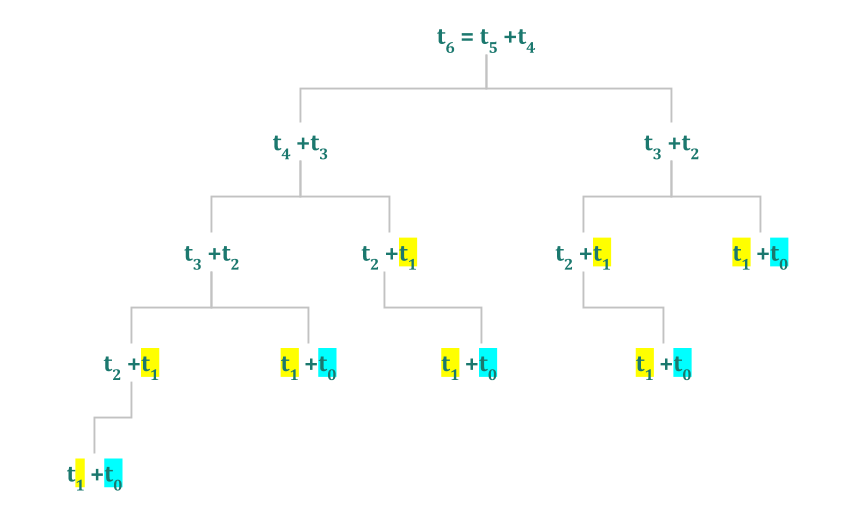
\includegraphics[scale=.4]{asst2_ques4}\\

\noindent b. Give an explicit formula for $t_n$:
\begin{flalign*}
&t_n = t_{n-1} + t_{n-2}\\
&\text{Rewrite as: } t_n - t_{n-1} - t_{n-2} = 0\\
&\text{Characteristic equation: } t^2 - t - 1 = 0\\
&\text{Characteristic roots: } \frac{1\pm\sqrt{1-4(-1)}}{2} = \frac{1\pm\sqrt{5}}{2}.\\
&t_n = a\left( \frac{1+\sqrt{5}}{2}\right)^n + b\left(\frac{1-\sqrt{5}}{2}\right)^n\\
&t_0 = a\left( \frac{1+\sqrt{5}}{2}\right)^0 + b\left(\frac{1-\sqrt{5}}{2}\right)^0 = a + b = 2\\
&t_1 =  a\left( \frac{1+\sqrt{5}}{2}\right)^1 + b\left(\frac{1-\sqrt{5}}{2}\right)^1 = \frac{a+b}{2} + \frac{(a-b)\sqrt{5}}{2} = 1\\
&\text{Since a+b=2, the first term of the last equation $\frac{a+b}{2}$ is equal to $\frac{2}{2}=1$.}\\
&\text{And so the second term $\frac{(a-b)\sqrt{5}}{2}$ must be equal to 0.}\\
&\text{Solving $a+b=2$ when $a-b=0$ results in $a=1$ and $b=1$.}\\
&\text{Thus, } t_n = \left( \frac{1+\sqrt{5}}{2}\right)^n + \left(\frac{1-\sqrt{5}}{2}\right)^n\\
\end{flalign*}
\end{document}